%%%% Supplementary Materials for main_v9.tex (IEEE OJEMB, 2026-08-30). Same artifacts as the
%%%% main text; every number is v8's. OJEMB allows up to 4,000 words and up to 10 display
%%%% items here; this file holds 3 tables (S-I..S-III) and 5 figures (S1..S5).
\documentclass[journal]{IEEEtran}
\usepackage[usenames]{color}
\usepackage{xcolor}
\usepackage{epsfig}
\usepackage{graphics}
\usepackage{caption}
\usepackage{amsmath}
\usepackage{amssymb}
\usepackage{multirow}
\usepackage{cite}
\usepackage{array}
\usepackage{pslatex}
\usepackage{url}
\usepackage{graphicx}
\usepackage{setspace}
\usepackage{hhline}
\usepackage{mathtools}
\usepackage{booktabs}
\usepackage{textcomp}
\usepackage[letterpaper]{geometry}
\geometry{verbose,tmargin=0.7in,bmargin=0.7in,lmargin=0.65in,rmargin=0.65in}
\setlength{\headheight}{17pt}
\setlength{\headsep}{5pt}
\captionsetup[figure]{name={Fig.},labelsep=period,font=small}
\captionsetup[table]{name={TABLE},labelsep=period,font=small}
\newcommand{\flogo}{
\includegraphics[height=18pt]{embLogo.eps}}
\usepackage[english]{babel}
\usepackage[utf8]{inputenc}
\usepackage{fancyhdr}
\pagestyle{fancy}
\fancyhf{}
\lhead{\textsc{\flogo}}
\rhead{\textcolor{violet}{\Large\textbf{Supplementary Materials}}}
\fancyfoot[C]{\thepage}
\renewcommand{\footrulewidth}{0.4pt}
\renewcommand{\thesection}{S-\Roman{section}}
\renewcommand{\thefigure}{S\arabic{figure}}
\renewcommand{\thetable}{S-\Roman{table}}
\graphicspath{{./}{Figures/}}
\newcolumntype{L}[1]{>{\raggedright\arraybackslash}p{#1}}

\begin{document}
\twocolumn[
\begin{@twocolumnfalse}
\thispagestyle{fancy}
\vspace*{0.5cm}
\textbf{\LARGE{Supplementary Materials}}\\
\\
\medskip\Large{Signal Quality, Representation, and Pre-Modelling Choices: A Measured Performance Budget for Surface-EMG Jaw-Activity Classification on Unseen Participants}\\
\normalsize{Mohammad~Hassan~Farhadi, Ali~Rabiee, Rahul~Singh, Mariusz~P.~Furmanek, Reza~Abiri*, and Theodore~A.~Walls*}\\
\vspace*{0.5cm}
\end{@twocolumnfalse}
]

\IEEEPARstart{T}{hese} Supplementary Materials are organised in the order in which the main text refers to them: the positioning comparison (Section~\ref{sec:s_positioning}), the protocol, dataset and configuration (Section~\ref{sec:s_protocol}), filter-chain selection (Section~\ref{sec:s_filter}), the RQ1 mechanism and the representation margin (Section~\ref{sec:s_rq1}), per-class curves and the learned representation (Section~\ref{sec:s_curves}), the secondary analyses (Section~\ref{sec:s_secondary}), the design constraints in detail (Section~\ref{sec:s_design}), training behaviour and cost (Section~\ref{sec:s_cost}), artifact provenance (Section~\ref{sec:s_provenance}) and author contributions (Section~\ref{sec:s_contrib}). Every number is regenerated from the same saved artifacts as the main text.

\section{Where This Study Stands}
\label{sec:s_positioning}

\subsection{Related Work}

Surface EMG is widely used for ambulatory assessment of masticatory activity because it measures muscle activation directly~\cite{raez2006techniques,farella2008masticatory}. Polysomnography with audio and video remains the reference standard for sleep bruxism~\cite{lavigne1996sleep,stuginski2016detection}, portable instruments show variable agreement with it~\cite{casett2017validity,cidverdejo2024instrumental}, and consensus guidance exists for ambulatory EMG~\cite{lobbezoo2020consensus}. Castroflorio et al.~\cite{castroflorio2013use,castroflorio2014detection} combined EMG and electrocardiographic information to identify sleep-bruxism episodes at home, and multi-day home recording is feasible~\cite{colonna2023electromyographic}. Machine-learning studies report high performance on controlled tasks, although labels, participants and validation protocols differ: Sonmezocak and Kurt~\cite{sonmezocak2021detection,sonmezocak2021machine} reported greater than 90\% accuracy from masseter-EMG features across relaxation, clenching, rhythmic grinding and fatigue or pain; Gul et al.~\cite{gul2024advanced} evaluated simulated sleep-bruxism activity across postures, Ishtiaq et al.~\cite{ishtiaq2025wearable} clenching detection from a two-muscle wearable, and Heyat et al.~\cite{heyat2020computational} and Tripathi et al.~\cite{tripathi2024computational} bruxism from public polysomnographic EEG and ECG; Lan et al.~\cite{lan2022comparative} described different surface-EMG patterns during centric and eccentric activities. Other sensing routes include mandibular movement~\cite{martinot2021artificial}, chin-mounted and in-ear inertial units~\cite{patwa2017bruxism,schlaepfer2026new,bondareva2021earables}, radar~\cite{shen2026bruxism}, contingent-stimulation devices~\cite{haugland2020automatic}, acoustic transducers~\cite{nahhas2024wearable} and temporalis EMG in eyeglasses~\cite{zhang2018monitoring}.

Wavelet decomposition suits EMG because muscle activity is non-stationary and a wavelet transform preserves when something happened as well as at what frequency~\cite{mallat1989theory,daubechies1992ten,englehart2003robust}; wavelet features perform well in EMG classification~\cite{phinyomark2012feature,bharathi2025unveiling}. Filter design remains important~\cite{chowdhury2013surface,deluca2010filtering,clancy2002sampling,merletti2020tutorial,boyer2023reducing}, and recording standards exist for electrode selection and amplitude normalisation~\cite{isek1999standards,hermens2000development,besomi2019consensus,besomi2020consensus,merletti2019tutorial}. Convolutional networks learn local patterns in physiological signals~\cite{faust2018deep,kiranyaz20211d}, an approach mature enough in myoelectric control to have public benchmarks~\cite{atzori2014electromyography,coteallard2019deep}.

Surface-EMG reviews identify powerline interference as the dominant environmental artifact and recommend a notch filter with a band-pass stage~\cite{chowdhury2013surface,raez2006techniques}, usually implemented as a single notch at the supply frequency. That is valid only when the supply fundamental is in fact the dominant interference. Mains wiring does not radiate a clean 60-Hz tone: lighting, displays and switched-mode supplies distort the waveform, so energy also appears at its harmonics inside the 20--450-Hz band that muscle activity occupies, and some acquisition systems apply a fixed notch of their own before the data reach the analysis software. Harmonic-aware methods have been available for two decades~\cite{mewett2004reducing,levkov2005removal,keshtkaran2014fast,sornmo2005bioelectrical}; they are simply not routine here, and nothing in a conventional analysis would say that they were needed. A scoping review of ambulatory EMG for bruxism found acquisition and analysis parameters reported inconsistently or not at all~\cite{thymi2021signal}, the same concern that drives reporting standards and leakage audits elsewhere in clinical machine learning~\cite{collins2024tripod,kapoor2023leakage,varoquaux2022machine,pineau2021improving}.

\subsection{Positioning}

Table~\ref{tab:positioning} places this study beside the machine-learning studies of jaw activity and bruxism it is most often compared with, and beside the alternative sensing routes. Three patterns are visible. Cohorts are small everywhere, three to thirty people, and most are healthy volunteers simulating the behaviour. Validation is usually pooled, so the reported accuracy describes recognition within the people recorded rather than transfer to a new one. And what a paper varies is almost always the classifier, sometimes the features, sensor or posture, and never the stages upstream of all of them; we found no study that publishes a measured statement about the signal that entered its pipeline, or that prices its segmentation or normalisation choices against its model. The only public recordings with a bruxism label are two overnight polysomnograms in the CAP Sleep Database~\cite{terzano2001atlas,goldberger2000physiobank}, whose EMG is submental and whose subjects are asleep. Against that background this study is one of the smaller cohorts and the only one recruited on a prior clinical diagnosis. It is also the only one in which the participant is the unit of validation throughout, a quiet-rest condition is included, the signal is measured before it is modelled, and the pipeline's stages are priced against each other. Table~\ref{tab:positioning} is a comparison, not a systematic review: its entries were checked against the sources, but the search was not exhaustive, and an unreported check is not proof of an absent one.

\begin{table*}[!t]
  \centering
  \caption{Where this study stands. Machine-learning studies of jaw activity and bruxism, and the alternative sensing routes, on the axes that determine what a reported accuracy means. ``Held-out participants'' states whether every test participant was absent from training; ``Varied'' lists what each study compared within itself. ``n.s.'': not stated in the source.}
  \label{tab:positioning}
  \footnotesize
  \begin{tabular*}{\textwidth}{@{\extracolsep{\fill}}L{0.13\textwidth}L{0.12\textwidth}L{0.11\textwidth}L{0.16\textwidth}L{0.12\textwidth}L{0.13\textwidth}L{0.07\textwidth}@{}}
    \toprule
    Study & Signal & Cohort & Conditions & Held-out participants & Varied & Data \\
    \midrule
    \multicolumn{7}{l}{\emph{Masticatory-muscle surface EMG}}\\
    Sonmezocak \& Kurt 2021~\cite{sonmezocak2021detection} & masseter sEMG & 10 volunteers & relaxed, clenching, rhythmic grinding, fatigue or pain; instructed & no: random split of segments & features, network settings & n.s. \\
    Gul et al.\ 2024~\cite{gul2024advanced} & bilateral temporalis and masseter sEMG & 10 healthy volunteers, simulating & rest, talking, chewing, clenching, grinding; three postures & no: 10-fold over windows, oversampled & classifier, muscle, posture & on request \\
    Ishtiaq et al.\ 2025~\cite{ishtiaq2025wearable} & temporalis and masseter sEMG, wearable & 30 volunteers, 5 trials each & clenching vs.\ other; supine & n.s.; oversampled & classifier, oversampling & n.s. \\
    Zhang \& Amft 2018~\cite{zhang2018monitoring} & temporalis sEMG in eyeglasses & 10 volunteers & chewing and eating vs.\ other; laboratory and 122~h free living & n.s. & setting, food hardness & n.s. \\
    Castroflorio et al.\ 2013, 2014~\cite{castroflorio2013use,castroflorio2014detection} & masseter sEMG and ECG holter, at home & 21 bruxers, 21 controls & sleep-bruxism episodes against polysomnography & per-participant agreement; rule-based & device vs.\ reference & n.s. \\
    \midrule
    \multicolumn{7}{l}{\emph{Other signals}}\\
    Heyat et al.\ 2020; Tripathi et al.\ 2024~\cite{heyat2020computational,tripathi2024computational} & overnight PSG: EEG, ECG, chin EMG & public database; 2 bruxism subjects available & bruxism vs.\ healthy; sleep stages & no: segment-level cross-validation & channel, classifier ensemble & public \\
    Martinot et al.\ 2021~\cite{martinot2021artificial} & mandibular movement, chin sensor & 67 suspected-OSA patients & phasic sleep bruxism against polysomnography & n.s. & device vs.\ reference & n.s. \\
    Bondareva et al.\ 2021~\cite{bondareva2021earables} & in-ear inertial unit & 13 volunteers & grinding, clenching vs.\ silent; still and while moving & yes: leave-one-out & sensor, classifier & n.s. \\
    Schlaepfer et al.\ 2026~\cite{schlaepfer2026new} & chin inertial unit & 3 volunteers, 21 recordings & grinding, opening and closing, other; simulated & no: pooled 80/20 split & classifier, sensor subset & on request \\
    Shen et al.\ 2026~\cite{shen2026bruxism} & 60-GHz radar & 3 volunteers, 180 clips & grinding vs.\ none & no: 10-fold over clips & classifier & n.s. \\
    \midrule
    \textbf{This study} & bilateral temporalis and masseter sEMG, 4 channels, archived as acquired with metadata & 5 adults with a prior clinical diagnosis & rest, movement, clenching, grinding, chewing of three foods; awake, instructed & \textbf{yes}: nested LOSO, 3 seeds & \textbf{signal chain, representation, architecture, window and context, normalisation scope} & on request \\
    \bottomrule
  \end{tabular*}
\end{table*}

\section{Protocol, Dataset and Configuration}
\label{sec:s_protocol}

\subsection{Why the Data Were Collected for This Study}

A stage-by-stage analysis makes demands of its data that a downloaded dataset rarely meets. Varying the filter chain (RQ1) requires the continuous recording as the acquisition system wrote it, with a record of what that system did to the signal before it reached disk. Pricing segmentation and temporal context (RQ4) requires a synchronised task marker with its timing preserved. Estimating false alarms requires a quiet non-event condition recorded with the same electrodes in the same session, which activity-only collections omit. Testing whether functional chewing confounds tooth-contact activity requires more than one food, because chewing rhythm and effort depend on food hardness~\cite{zhang2018monitoring}. And a held-out-participant evaluation requires that every channel of every recording belong to the participant it is labelled with, which only the raw files can verify. Searches of PhysioNet, Zenodo and Mendeley Data on 25 August 2026 returned no dataset of masticatory-muscle EMG during jaw activity; the only public recordings with a bruxism label are the two CAP Sleep Database polysomnograms, and the masticatory-EMG studies of Table~\ref{tab:positioning} each collected their own data, none of it public. None of the protocol's elements is novel on its own: bilateral masseter and temporalis recording is the standard montage~\cite{ferrario2000electromyographic,castroflorio2005reproducibility}, and instructed clenching, grinding and chewing tasks appear in several studies in Table~\ref{tab:positioning}. What is unusual is the combination: five conditions including quiet rest, non-contact movement and three foods, in adults with a prior clinical diagnosis rather than volunteers simulating the behaviour, four channels, a synchronised marker, a camera for review, and every channel of every recording archived as acquired with the acquisition software's own settings. That last choice made the filter defect discoverable a year after the sessions, and correctable without re-recording anyone.

\subsection{Participants and Procedure}

Five adults (two women and three men; age $38.0 \pm 10.4$ years) were recruited through flyers, local oral-care and physical-therapy providers, and word of mouth. Eligibility required a prior clinical diagnosis of bruxism, which the study did not re-diagnose or phenotype, so the diagnosis describes the sample and is not a reference standard for the activity labels. All tasks were performed intentionally while participants were awake in the laboratory; no spontaneous episodes and no sleep were recorded. Participants completed 1~min of quiet rest; five repetitions each of jaw opening and closing, left and right deviation, protrusion and retrusion, and left and right biting; and 1-min trials of isometric molar and incisor clenching alternating 3~s of activity with 3~s of relaxation. After a break they completed three 1-min trials each of instructed grinding, chewing cheese, chewing baby carrots or popcorn, and chewing gum. Every recording was 60~s long by design and held one condition, twenty recordings per participant; two ran short, at 52 and 41~s. A handheld button transmitted event markers synchronised with the recordings, pressed by the participant at task initiation and visually confirmed by the experimenter; these button-marked intervals are the sole source of the class labels. Four differential surface-EMG channels were recorded from bilateral bipolar electrode pairs over the masseter and temporalis on each side. A camera assisted offline review. A microphone was also recorded; it enters only the RQ1 contrast (main text, Table~I), as a fifth input channel in both of that contrast's arms, and no other reported number. All signals were sampled at 1200~Hz and written to disk as acquired, as a six-column file with a metadata sidecar recording the acquisition software's own filter settings; nothing was resampled, filtered or segmented at collection time. The acquisition chain documented no physical calibration, so amplitudes are reported in arbitrary analog-to-digital converter units rather than microvolts, and electrode type, amplifier, gain and converter resolution are not documented, short of current reporting recommendations~\cite{isek1999standards,besomi2019consensus}.

\subsection{Window Labelling and the Analysable Sample}

Every analysed window lies wholly inside one trigger-marked task interval, so no window spans two conditions or a trigger transition. Windows are cut from the continuously filtered recording and never filtered individually, which would inject an edge transient into each window. Three exclusions are applied before windowing, each measured rather than assumed (Table~\ref{tab:dataset}). A transition guard of 0.25~s is removed on each side of every trigger edge: over 432 task onsets, muscle activity preceded the marker at 79.9\%, and among the remainder the median lag was 0.054~s and the largest 0.352~s, so the guard covers the 95th percentile of the harmful direction. A startup guard of 0.5~s is removed at the beginning of every recording, because amplifier settling transients appeared in 66 of 100 recordings and all settled within 0.40~s. Quiet-rest windows are drawn only from the five dedicated rest recordings, because trigger-off intervals inside active recordings are unlabelled rather than verified as quiet; the rest class therefore represents quiet laboratory rest, not everyday non-event behaviour.

The recordings were consolidated into five classes: rest, the dedicated quiet-baseline recordings; movement, opening and closing, lateral deviation, protrusion and retrusion; clenching, molar and incisor clench and unilateral bite; grinding; and chewing of cheese, carrots or popcorn, and gum. Bracing and thrusting without tooth contact were not elicited. Chewing was included as a common functional activity and a plausible confound for an ambulatory classifier; because it may also be comparatively easy to recognise, the five-class results are accompanied by a sensitivity analysis that excludes it and by one that collapses the labels into clenching or grinding versus the rest (Section~\ref{sec:s_secondary}). Under these rules, 100 recordings yielded 6,173 analysable 1.0-second windows from 99 recordings. Class sizes are strongly unequal: chewing supplies 58.9\%, and within a class the counts differ between participants because they marked the trigger differently (Section~\ref{sec:s_design}). The windows are not independent observations, adjacent windows overlapping by 50\% and all coming from five people, so the participant is the unit for generalisation and all primary metrics are computed within a participant before being summarised~\cite{saeb2017need,little2017using,roberts2017cross}.

\subsection{Training and Evaluation Details}

Class imbalance was addressed with inverse-frequency class weights recomputed within each outer training fold, and with augmentation of minority-class training windows by amplitude scaling, additive noise and circular shifts, confined structurally to the training partition; the settings are in Table~\ref{tab:dataset}. Nested LOSO was used because selecting a model and reporting its score on the same held-out data biases the estimate upward~\cite{cawley2010overfitting,varma2006bias}; macro-F1 was the selection objective because accuracy is dominated by chewing~\cite{chicco2020advantages}; and each outer fold's epoch budget is the median of its inner folds' best epochs (15--43). Accuracy, balanced accuracy, macro precision, recall, F1 and one-vs-rest ROC--AUC are computed within each held-out participant and then summarised across the five; pooled-window metrics are descriptive only, because windows within a participant are correlated. No window-level bootstrap intervals or $p$-values are reported: the windows are clustered and overlapping, and with five participants such tests would overstate precision without supporting a population-level claim~\cite{lehmann2006testing,demsar2006statistical}. Held-out probabilities are uncalibrated (expected calibration error 0.063) and must not be read as probabilities~\cite{guo2017calibration}; every AUC, being rank-based, is unaffected. The per-participant, or transductive, normalisation scope is implemented and priced in Section~\ref{sec:s_design}, but no confirmatory number uses it: the strict scope is the one that would support a deployment claim without a fitting session~\cite{besomi2020consensus}.

\begin{table}[!t]
  \caption{Dataset, guards, preprocessing and training configuration under the trigger-constrained labelling policy.}
  \label{tab:dataset}
  \centering
  \footnotesize
  \begin{tabular*}{\columnwidth}{@{\extracolsep{\fill}}ll@{}}
    \toprule
    Property & Value \\
    \midrule
    \multicolumn{2}{l}{\emph{Dataset and guards}}\\
    Participants / recordings & 5 / 100 (99 analysable) \\
    EMG channels analysed & 4 (2 bilateral pairs) \\
    Sampling rate / units & 1200 Hz / arbitrary ADC \\
    Window / stride & 1200 (1.0 s) / 600 (0.5 s) \\
    Transition guard, per edge & 0.25 s \\
    Startup guard, per recording & 0.5 s \\
    Rest / movement windows & 590 / 333 \\
    Clenching / grinding windows & 799 / 816 \\
    Chewing windows & 3,635 \\
    \textbf{Total analysed windows} & \textbf{6{,}173} \\
    \midrule
    \multicolumn{2}{l}{\emph{Preprocessing}}\\
    Mains notches (8 Hz wide) & 60--420 Hz, 7 harmonics \\
    Band-pass (Butterworth, order 4) & 20--450 Hz \\
    Filtering mode & Zero-phase, whole recording \\
    Wavelet / bands & db4, 4 levels / $A_4$, $D_3$, $D_1$ \\
    Normalisation scope & Strict (outer-train participants) \\
    \midrule
    \multicolumn{2}{l}{\emph{Training and evaluation}}\\
    Optimiser & AdamW \\
    Learning rate / weight decay & $10^{-3}$ / $10^{-4}$ \\
    Loss & Focal, $\gamma = 1.5$ \\
    Class weights & Inverse frequency, per fold \\
    Dropout / batch size & 0.5 / 64 \\
    Gradient clipping & Norm 1.0 \\
    Epoch budget & Median inner best (15--43) \\
    Seeds & 0, 1, 2 \\
    Outer / inner folds & 5 / 4, participant-grouped \\
    \bottomrule
  \end{tabular*}
\end{table}

\section{Filter-Chain Selection and Preprocessing}
\label{sec:s_filter}

Across all 100 recordings, 62 had more than 30\% of their raw in-band EMG power within $\pm3$~Hz of a mains multiple, and in the five quiet-rest recordings that share was 91.3--99.8\%. Through the superseded chain, a single 60-Hz notch ($Q=30$) followed by a 20--450-Hz band-pass, the mains share of in-band power after filtering was 91.4--99.8\%, essentially unchanged; a filter-response plot of that chain looks entirely conventional, which is why the problem stayed invisible until the response was drawn over the measured spectrum of the data (main text, Fig.~2). The corrected chain's pass band is consistent with direct measurements of jaw and facial EMG~\cite{vanboxtel2001optimal,deluca2010filtering}. Each notch is constant-width, 8~Hz at $-3$~dB, rather than constant-$Q$: at an identical 13\% band cost the constant-width bank left eight times less residual interference, and after correction the mains share in the quiet-rest recordings fell to 0.46--0.66\%. The chain was selected on this interference criterion, which can be specified in advance, and not on held-out score; the distinction is not decorative, because the constant-$Q$ bank scored marginally higher in screening classification, at 0.689 against 0.679 macro-F1, while leaving eight times the interference. All filtering is zero-phase and applied to the whole continuous recording before any window is cut; it suits offline analysis and cannot support a streaming claim. The pipeline rejects any wavelet band its own filter chain has removed unless the configuration declares the exception, which is why $D_1$ is used only over 300--450~Hz. Fig.~\ref{fig:preprocessing} shows the chain on a real excerpt.

\begin{figure*}[!t]
  \centering
  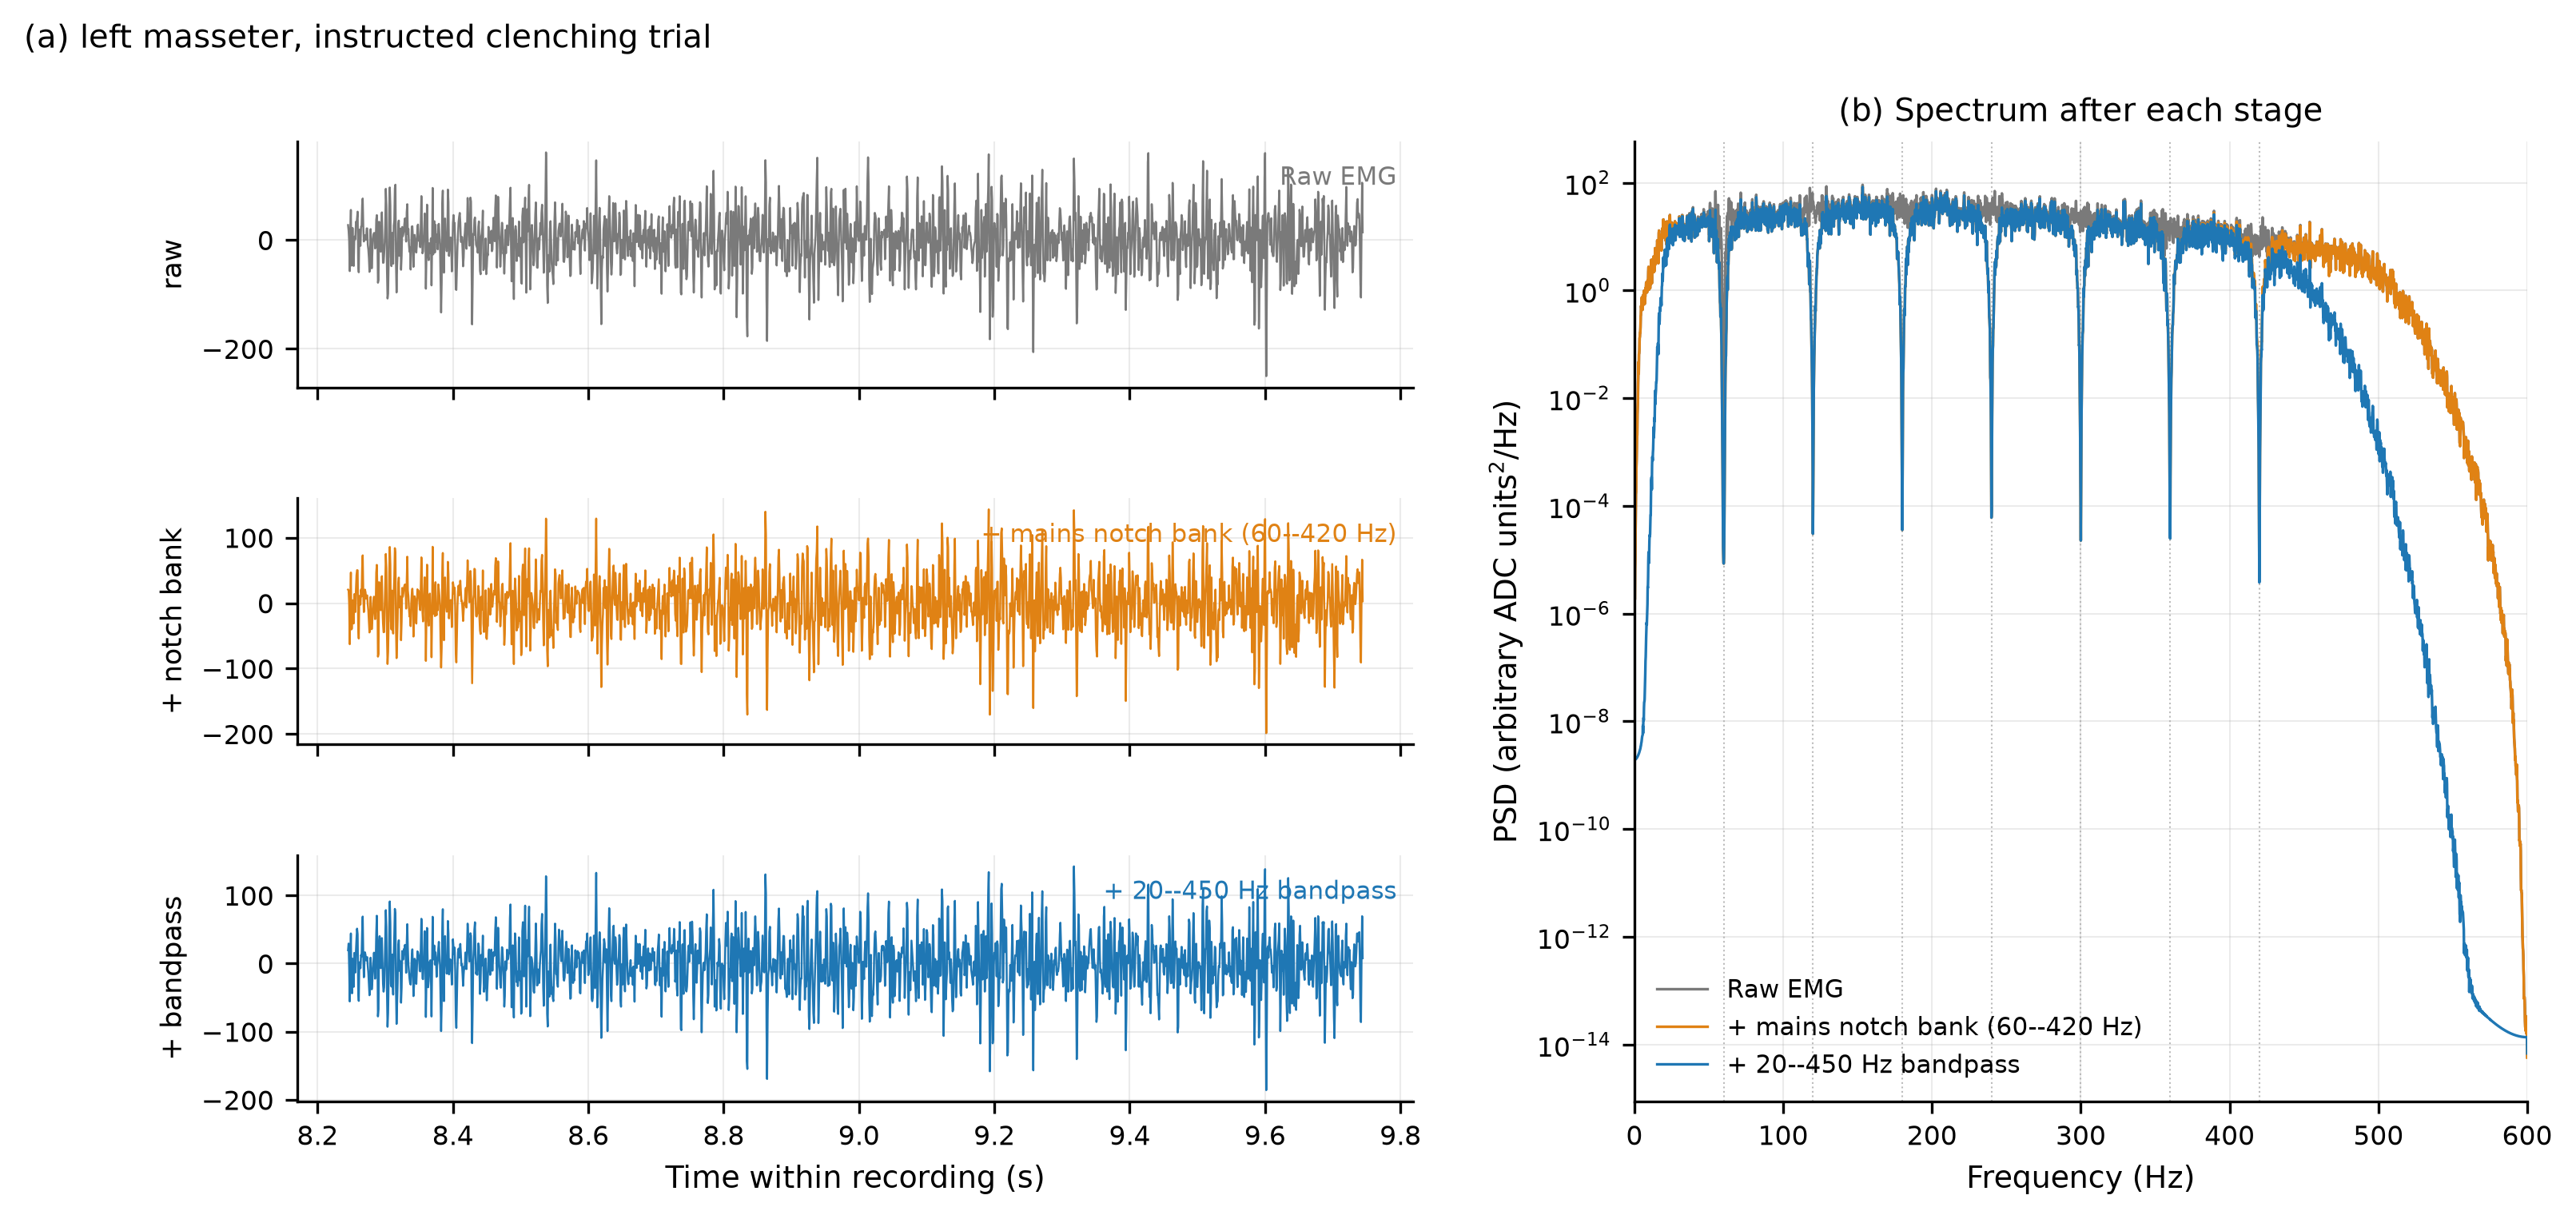
\includegraphics[width=0.84\textwidth]{Figures/preprocessing_stages_5class.png}
  \caption{Production preprocessing on a real excerpt of an instructed clenching trial (left masseter channel). (a) Time domain and (b) power spectrum after each stage: the notch bank removes the seven mains multiples marked by dotted lines, and the band-pass then removes content outside 20--450~Hz. The chain is applied to the continuous recording; windows are cut afterwards.}
  \label{fig:preprocessing}
\end{figure*}

\section{RQ1 in Signal Terms, and the Representation Margin}
\label{sec:s_rq1}

The RQ1 comparison (main text, Table~I) holds the 6,173 windows, their fold assignments and their labels identical in both arms, verified by comparing the two prediction ledgers window by window. The screening harness reproduces the effect with two much simpler estimators: logistic regression on the 28 band-energy features moved from 37.3\% to 63.9\% macro-F1, and gradient boosting from 38.8\% to 61.3\%. Through the superseded chain two of the five held-out participants were essentially unclassifiable, P1 at 18.1\% macro-F1 and P2 at 5.4\%, at or below a constant prediction, while P3 to P5 scored 57.6--75.4\%; after the correction the same five span 61.4--82.4\%. What had looked like severe between-participant heterogeneity was substantially an artifact of interference differing between recording sessions.

Three further measurements show that the superseded chain was inert rather than merely suboptimal, and explain the mechanism (Fig.~\ref{fig:measurement_chain}). First, a control chain with no mains removal at all scored 38.5\% macro-F1 in screening, within 1.2 points of the superseded chain: filtering a fundamental the hardware had already removed was equivalent to not filtering. Second, the interference was the dominant signal. Expressed as each activity's median RMS divided by that participant's own resting RMS, the contrast a classifier must exploit, the superseded chain left chewing at 1.6--7.2$\times$ rest and clenching at 1.6--5.2$\times$; after correction the same quantities are 8.5--35.7$\times$ and 8.1--27.0$\times$. Third, the superseded chain left a 5.07$\times$ spread between the largest and smallest participant median RMS and 20 pairs in which one person's resting EMG exceeded another's active EMG, against 2.97$\times$ and none after correction. Two features bound the contrast in opposite directions: the superseded arm carried an extra input channel and searched its hyperparameters, making the gap conservative; but the two runs differ in codebase version, and although the windows, folds and labels are byte-identical and were verified as such, an unrecorded contributing difference cannot be excluded. The screening arms share one code path across both chains and are the cleaner evidence on that specific point.

\begin{figure*}[!t]
  \centering
  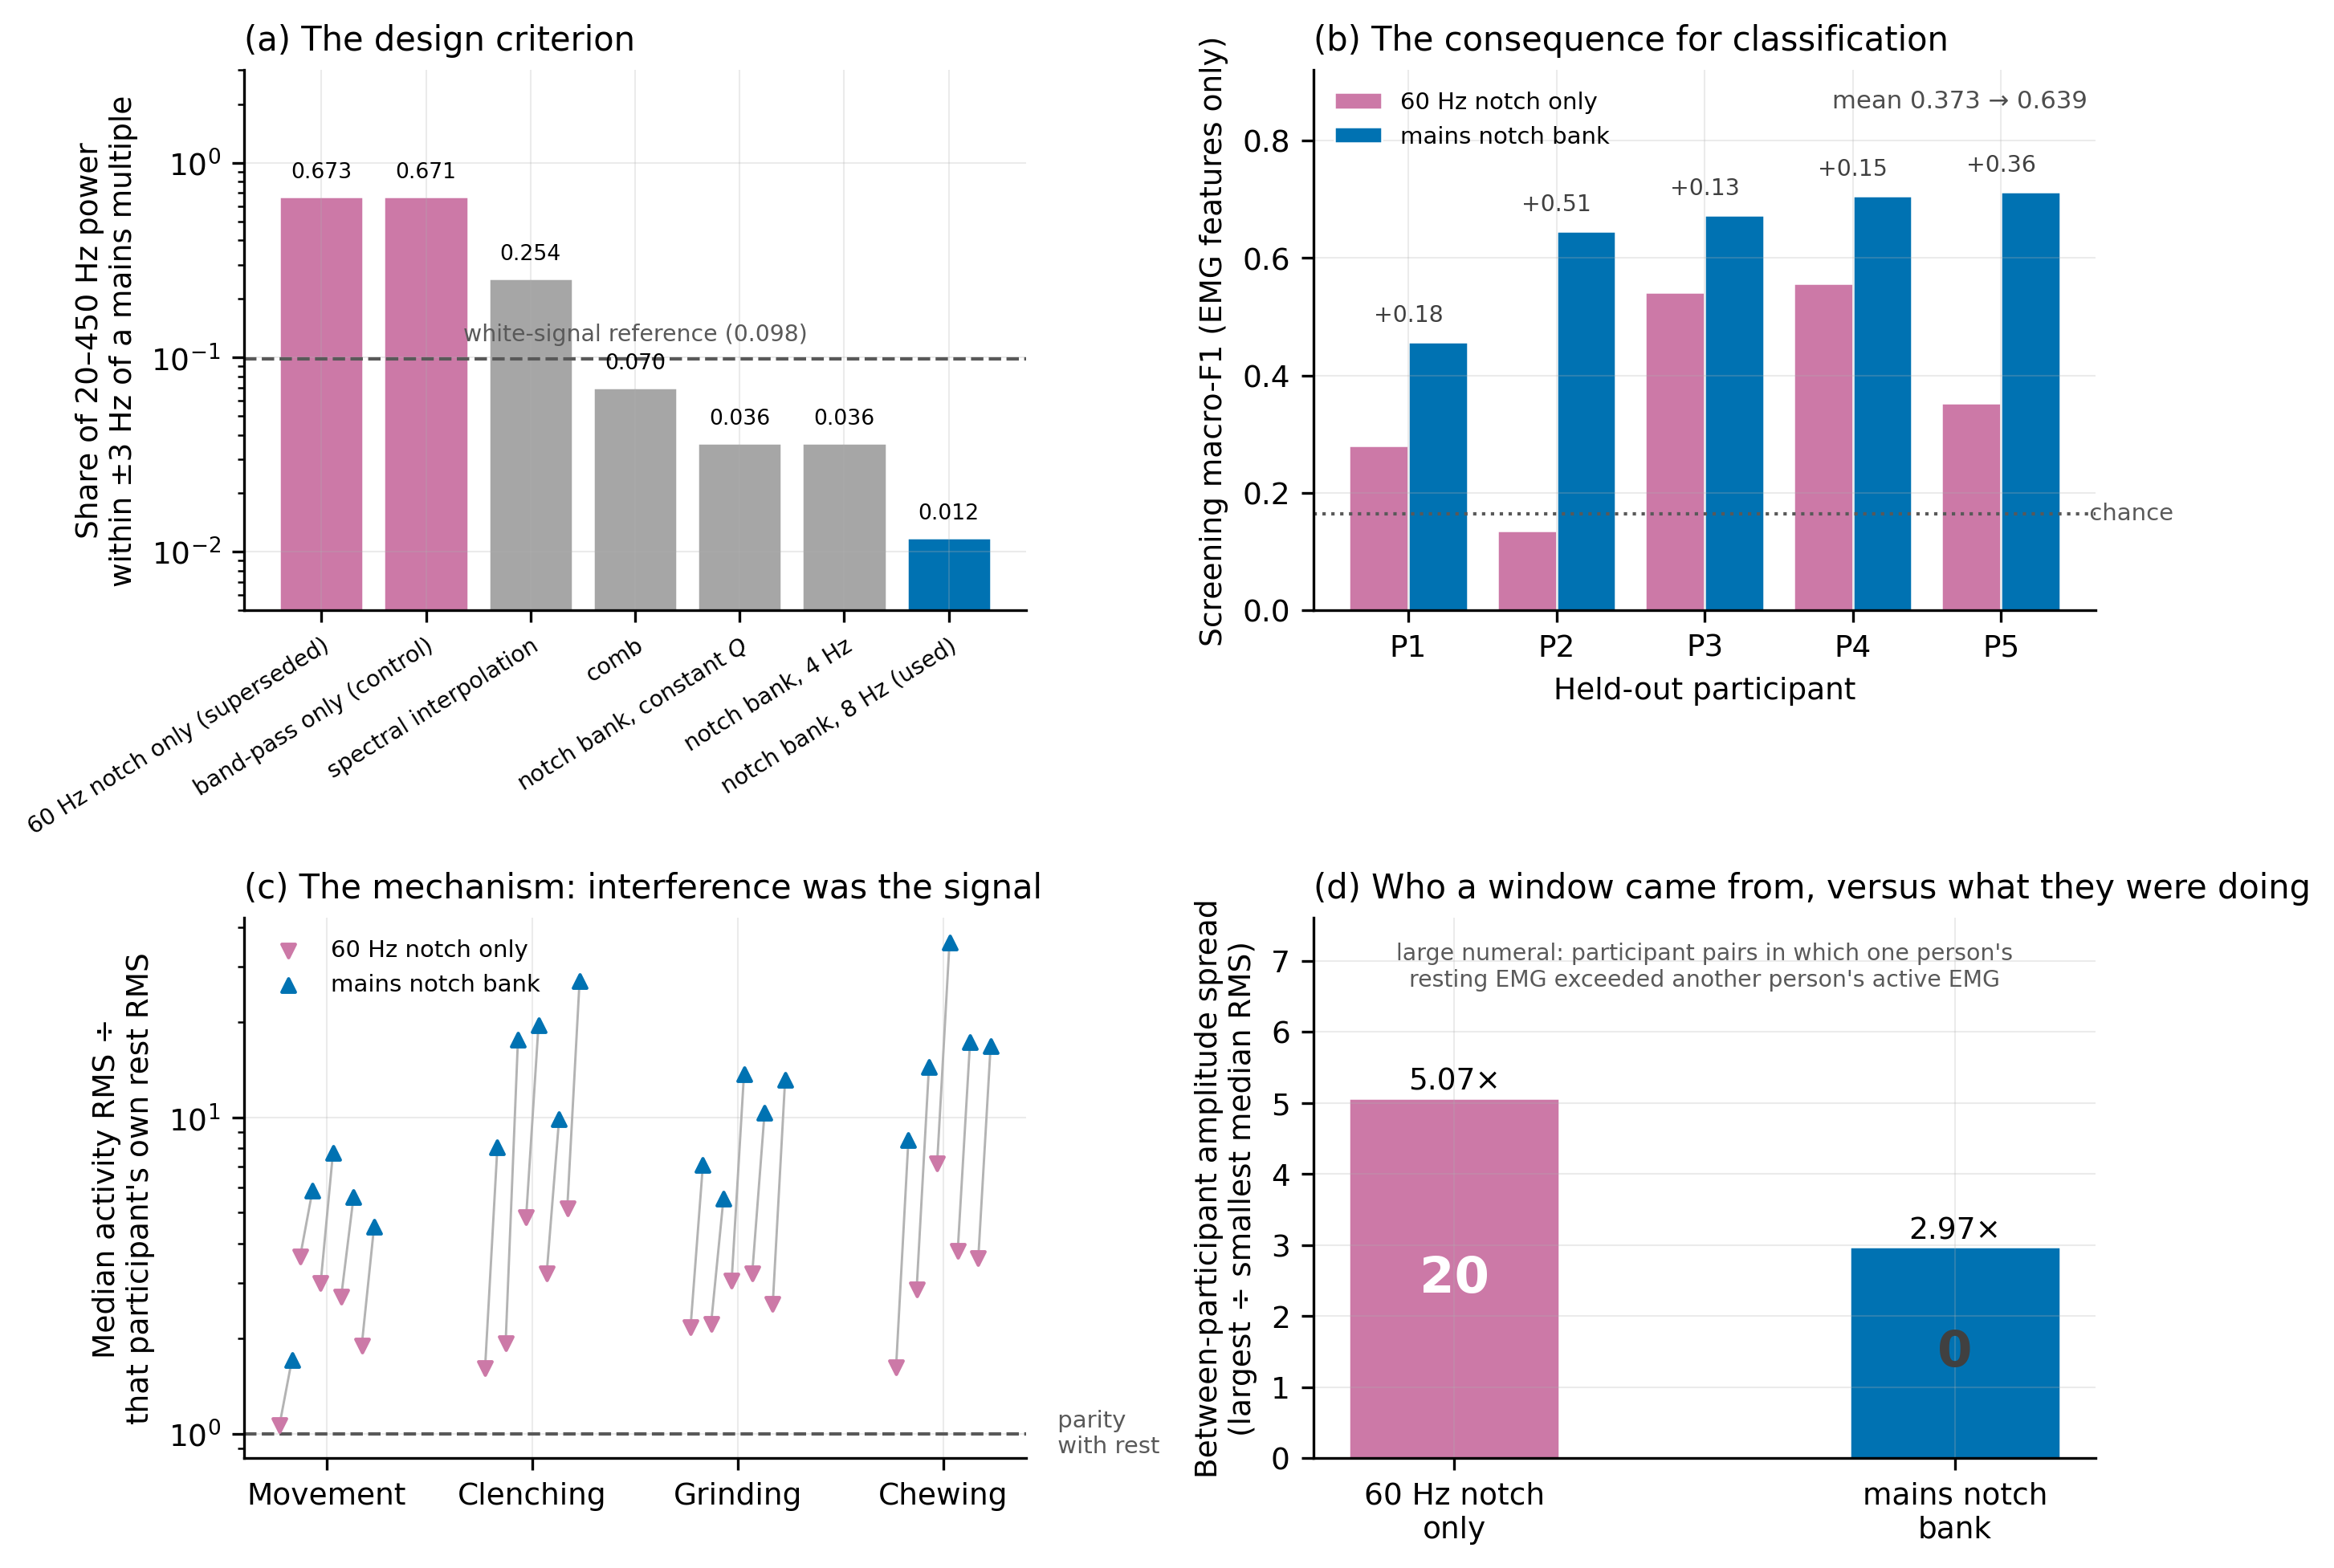
\includegraphics[width=0.86\textwidth]{Figures/v5/measurement_chain.png}
  \caption{The mains-harmonic defect in classification terms. (a) Residual mains power for every candidate chain, against the 0.098 a white signal would score. (b) Screening macro-F1 per held-out participant before and after the correction. (c) Each activity's median RMS divided by that participant's own resting RMS, before (down triangles) and after (up triangles). (d) Between-participant amplitude spread and the number of pairs in which one person's resting EMG exceeded another's active EMG.}
  \label{fig:measurement_chain}
\end{figure*}

\subsection{The Representation Margin}

The network's 8.1- and 10.6-point margins over the two screening baselines (main text, Table~II) are stable in direction across two very different estimators, but the AUC column does not follow: logistic regression reaches a participant-level macro AUC of 0.965 against the network's 0.958, a difference smaller than the network's own seed-to-seed range, so the two models rank held-out windows about equally well and the network's advantage lies in where its decision boundaries fall. That is why macro-F1 rather than AUC was the prespecified selection objective. One qualification matters more than the margin: the advantage was much smaller before the measurement chain was corrected. Through the superseded chain the network reached 43.5\% macro-F1 against 39.3\% and 40.1\% for the two baselines, a margin of about four points obtained by a network that additionally searched its hyperparameters and carried a microphone branch. The near-parity had been read as evidence that the architecture contributed nothing over band energies; the reading was correct about the numbers and wrong about the cause. When the dominant variance in a window is interference amplitude, a per-band pooled amplitude is all there is to extract, and a network whose sub-branches compute pooled band amplitudes cannot beat features that compute them directly. Once the interference is removed the margin roughly doubles.

\section{Per-Class Curves and the Learned Representation}
\label{sec:s_curves}

Fig.~\ref{fig:roc_tsne}(a) shows the one-vs-rest ROC curves of seed 0, chosen by the fixed rule of lowest seed index because a curve drawn over pooled seeds would mix models; three-seed means are in Table~II of the main text. Movement reaches an AUC of 0.937, almost identical to clenching's 0.936, yet its precision is 34.4\% against clenching's 70.5\%; AUC is insensitive to class size and precision is not~\cite{saito2015precision,davis2006relationship}, so a reader who looks only at AUC will overestimate how usable the small classes are. Fig.~\ref{fig:roc_tsne}(b) is a t-SNE~\cite{vandermaaten2008visualizing} of the 32-dimensional penultimate representation for the held-out windows of one seed, so that each held-out window appears exactly once. It reproduces both error patterns of the confusion matrix: chewing occupies several well-separated regions, rest forms tight islands, clenching and grinding interleave, and movement scatters along the borders of the larger classes. t-SNE distances are not metric, so the embedding is corroboration only.

\begin{figure*}[!t]
  \centering
  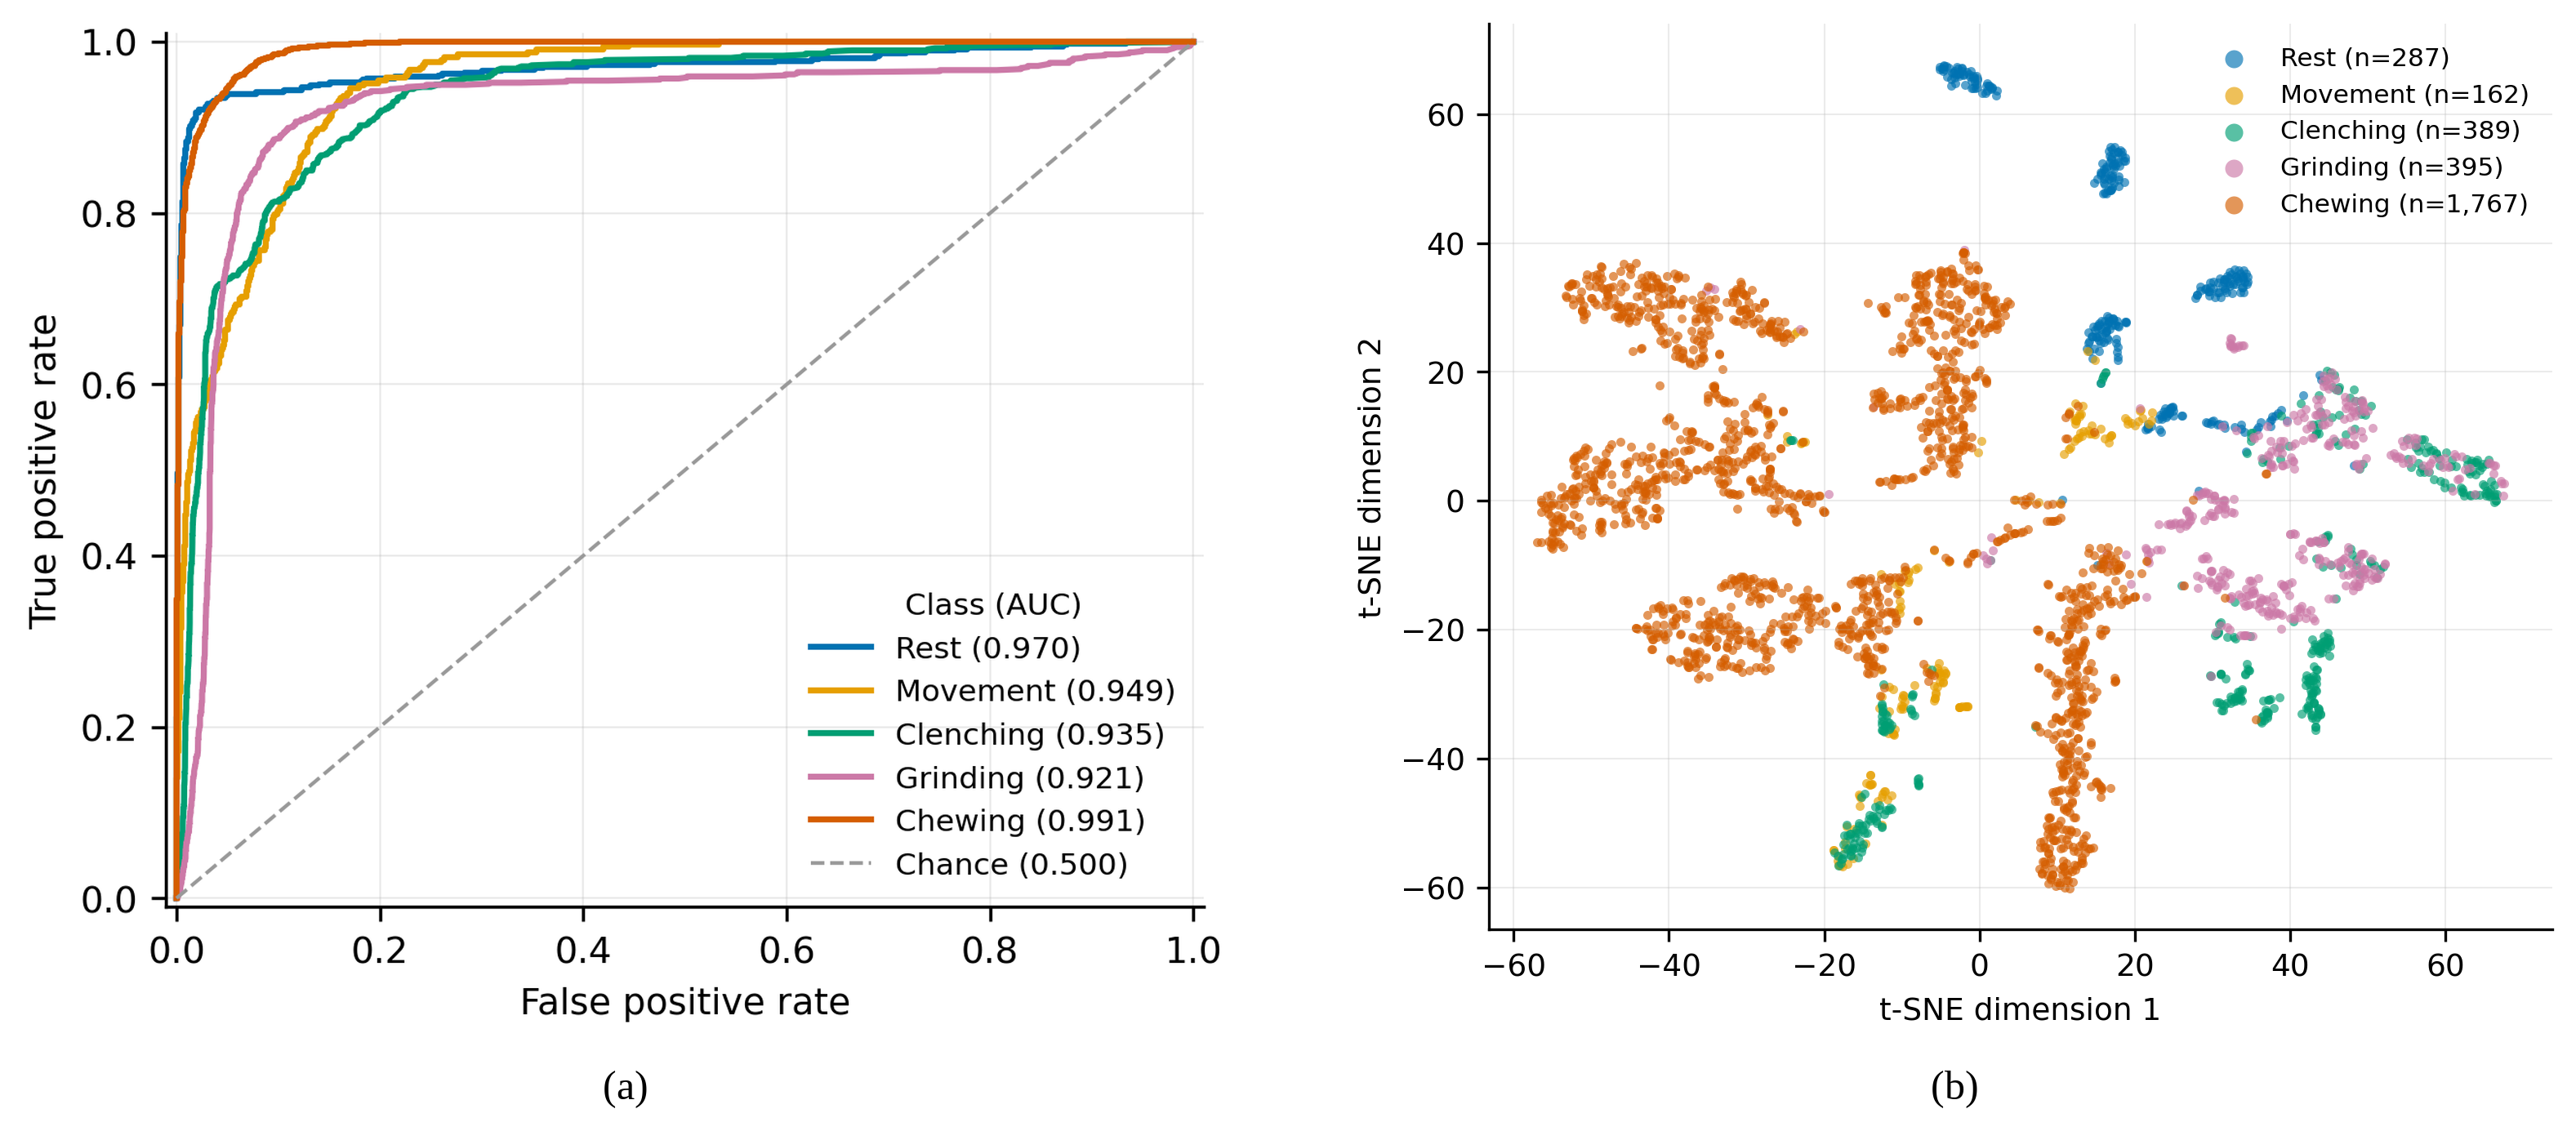
\includegraphics[width=0.86\textwidth]{Figures/v9/figS_roc_tsne.png}
  \caption{(a) One-vs-rest ROC curves for the five classes, pooled over the held-out windows of seed 0; legend values are that seed's. (b) t-SNE of the 32-dimensional penultimate representation for the held-out windows of one seed, coloured by class.}
  \label{fig:roc_tsne}
\end{figure*}

\section{Secondary Analyses}
\label{sec:s_secondary}

Two secondary analyses were computed post hoc from the same held-out predictions (Table~\ref{tab:sensitivity}): chewing windows removed and the remaining four probabilities renormalised, checked against a separately trained four-class model; and predictions collapsed into instructed clenching or grinding versus rest, movement and chewing. Both re-read one model, and the second is task discrimination, not bruxism detection. Excluding chewing leaves a four-class problem that yielded 77.7\% accuracy, 75.7\% macro-F1 and a macro AUC of 0.942 at participant level. Removing chewing lowers accuracy by 4.0 points but raises macro-F1 by 3.7, because the metric is no longer dominated by one large, easily separated class; a model trained separately on the same four classes reaches 75.8\% macro-F1, confirming that the post-hoc values are not an artifact of renormalisation. Treating clenching and grinding as the positive group yielded 92.5\% accuracy, 84.8\% sensitivity, 95.3\% specificity and an AUC of 0.970 on pooled windows, and 93.0\% accuracy with a participant-level macro-F1 of 89.3\%. Within the quiet-rest condition, 7.7\% of rest windows (45, 50 and 42 of 590 across the three seeds) fell on the tooth-contact side. At a 0.5-s decision interval that corresponds to roughly 550 false alarms per hour if the background were quiet rest throughout, a quantity this design cannot estimate, because rest was recorded in a controlled laboratory and did not sample speaking, swallowing, facial expression or head movement.

\begin{table*}[!t]
  \caption{Secondary analyses computed post hoc from the held-out five-class predictions, averaged over three seeds. These re-read one trained model; they are not separately trained tasks.}
  \label{tab:sensitivity}
  \centering
  \footnotesize
  \begin{tabular*}{\textwidth}{@{\extracolsep{\fill}}lcccccc@{}}
    \toprule
    Analysis & Accuracy & Precision & Recall & Specificity & F1 & AUC \\
    \midrule
    Excluding chewing$^{a}$ & 75.4\% & 74.9\% & 76.1\% & --- & 75.4\% & 0.919 \\
    Collapsed binary$^{b}$ & 92.5\% & 86.4\% & 84.8\% & 95.3\% & 85.5\% & 0.970 \\
    \bottomrule
  \end{tabular*}
  \begin{flushleft}\footnotesize
  Values are pooled over held-out windows; the participant-level means are 77.7\% accuracy, 75.7\% macro-F1 and 0.942 AUC excluding chewing, and 93.0\%, 89.3\% and 0.968 for the collapsed binary analysis.
  $^{a}$Macro values across rest, movement, clenching and grinding after removing chewing windows and renormalising the remaining probabilities.
  $^{b}$Instructed clenching and grinding treated as positive; rest, movement and chewing as the comparison group. Task discrimination, not clinical diagnosis.
  \end{flushleft}
\end{table*}

\section{Design Constraints in Detail}
\label{sec:s_design}

All three measurements are screening measurements on the identical 6,173 windows and five outer folds (main text, Fig.~4).

\textit{Temporal context.} Chewing and grinding are distinguished from clenching partly by rhythm, burst and relaxation cycles at roughly 1--2~Hz (Fig.~\ref{fig:signal_comparison}), which a 1.0-s window can barely contain. Averaging held-out probabilities over consecutive windows raises screening macro-F1 monotonically from 0.730 at 1.0~s of context to 0.769 at 2.5~s and 0.804 at 5.5~s, before flattening. The 7.4-point gain is a trial-level secondary analysis, because every recording holds a single condition, so averaging within a recording approaches a majority vote over a homogeneous trial: valid evidence that one second is too short, invalid as continuous-stream detection. The sweep was run under the per-participant normalisation scope, so its 1.0-s starting value of 0.730 is the value that scope earns; the two rows of the budget share a baseline and must not be summed.

\textit{Window, guard and trigger use.} Participants marked trigger intervals at very different granularity, 67 runs of median 8.7~s for P1 against 167 runs of median 1.7~s for P2, and a 1.0-s window with a 0.25-s guard on each side needs a run longer than 1.5~s to emit one window; P1's clenching trials emit 376 windows, P2's 53, and P2's movement trials 11. Sweeping only the guard from 0 to 0.5~s moves the smallest participant-and-class cell from 50 windows to 1, whereas a 0.5-s window with a 0.1-s guard yields 13,983 windows and a smallest cell of 128. The reported policy is a compromise; the real resolution is to standardise trigger use at collection time.

\textit{Normalisation scope.} Under the strict scope used for every confirmatory number, the screening classifier reaches 0.639 macro-F1; standardising each participant's features by that participant's own unlabelled distribution raises it to 0.730, a gain of 9.1 points. This is transductive test-time adaptation, not label leakage, but it presumes a per-user fitting session and therefore describes a different product, so it is excluded from every reported result~\cite{besomi2020consensus}. Normalising per recording instead destroys the task, at 0.036 macro-F1, because each recording holds one condition and per-recording standardisation removes precisely the between-condition amplitude difference the task depends on.

\begin{figure*}[!t]
  \centering
  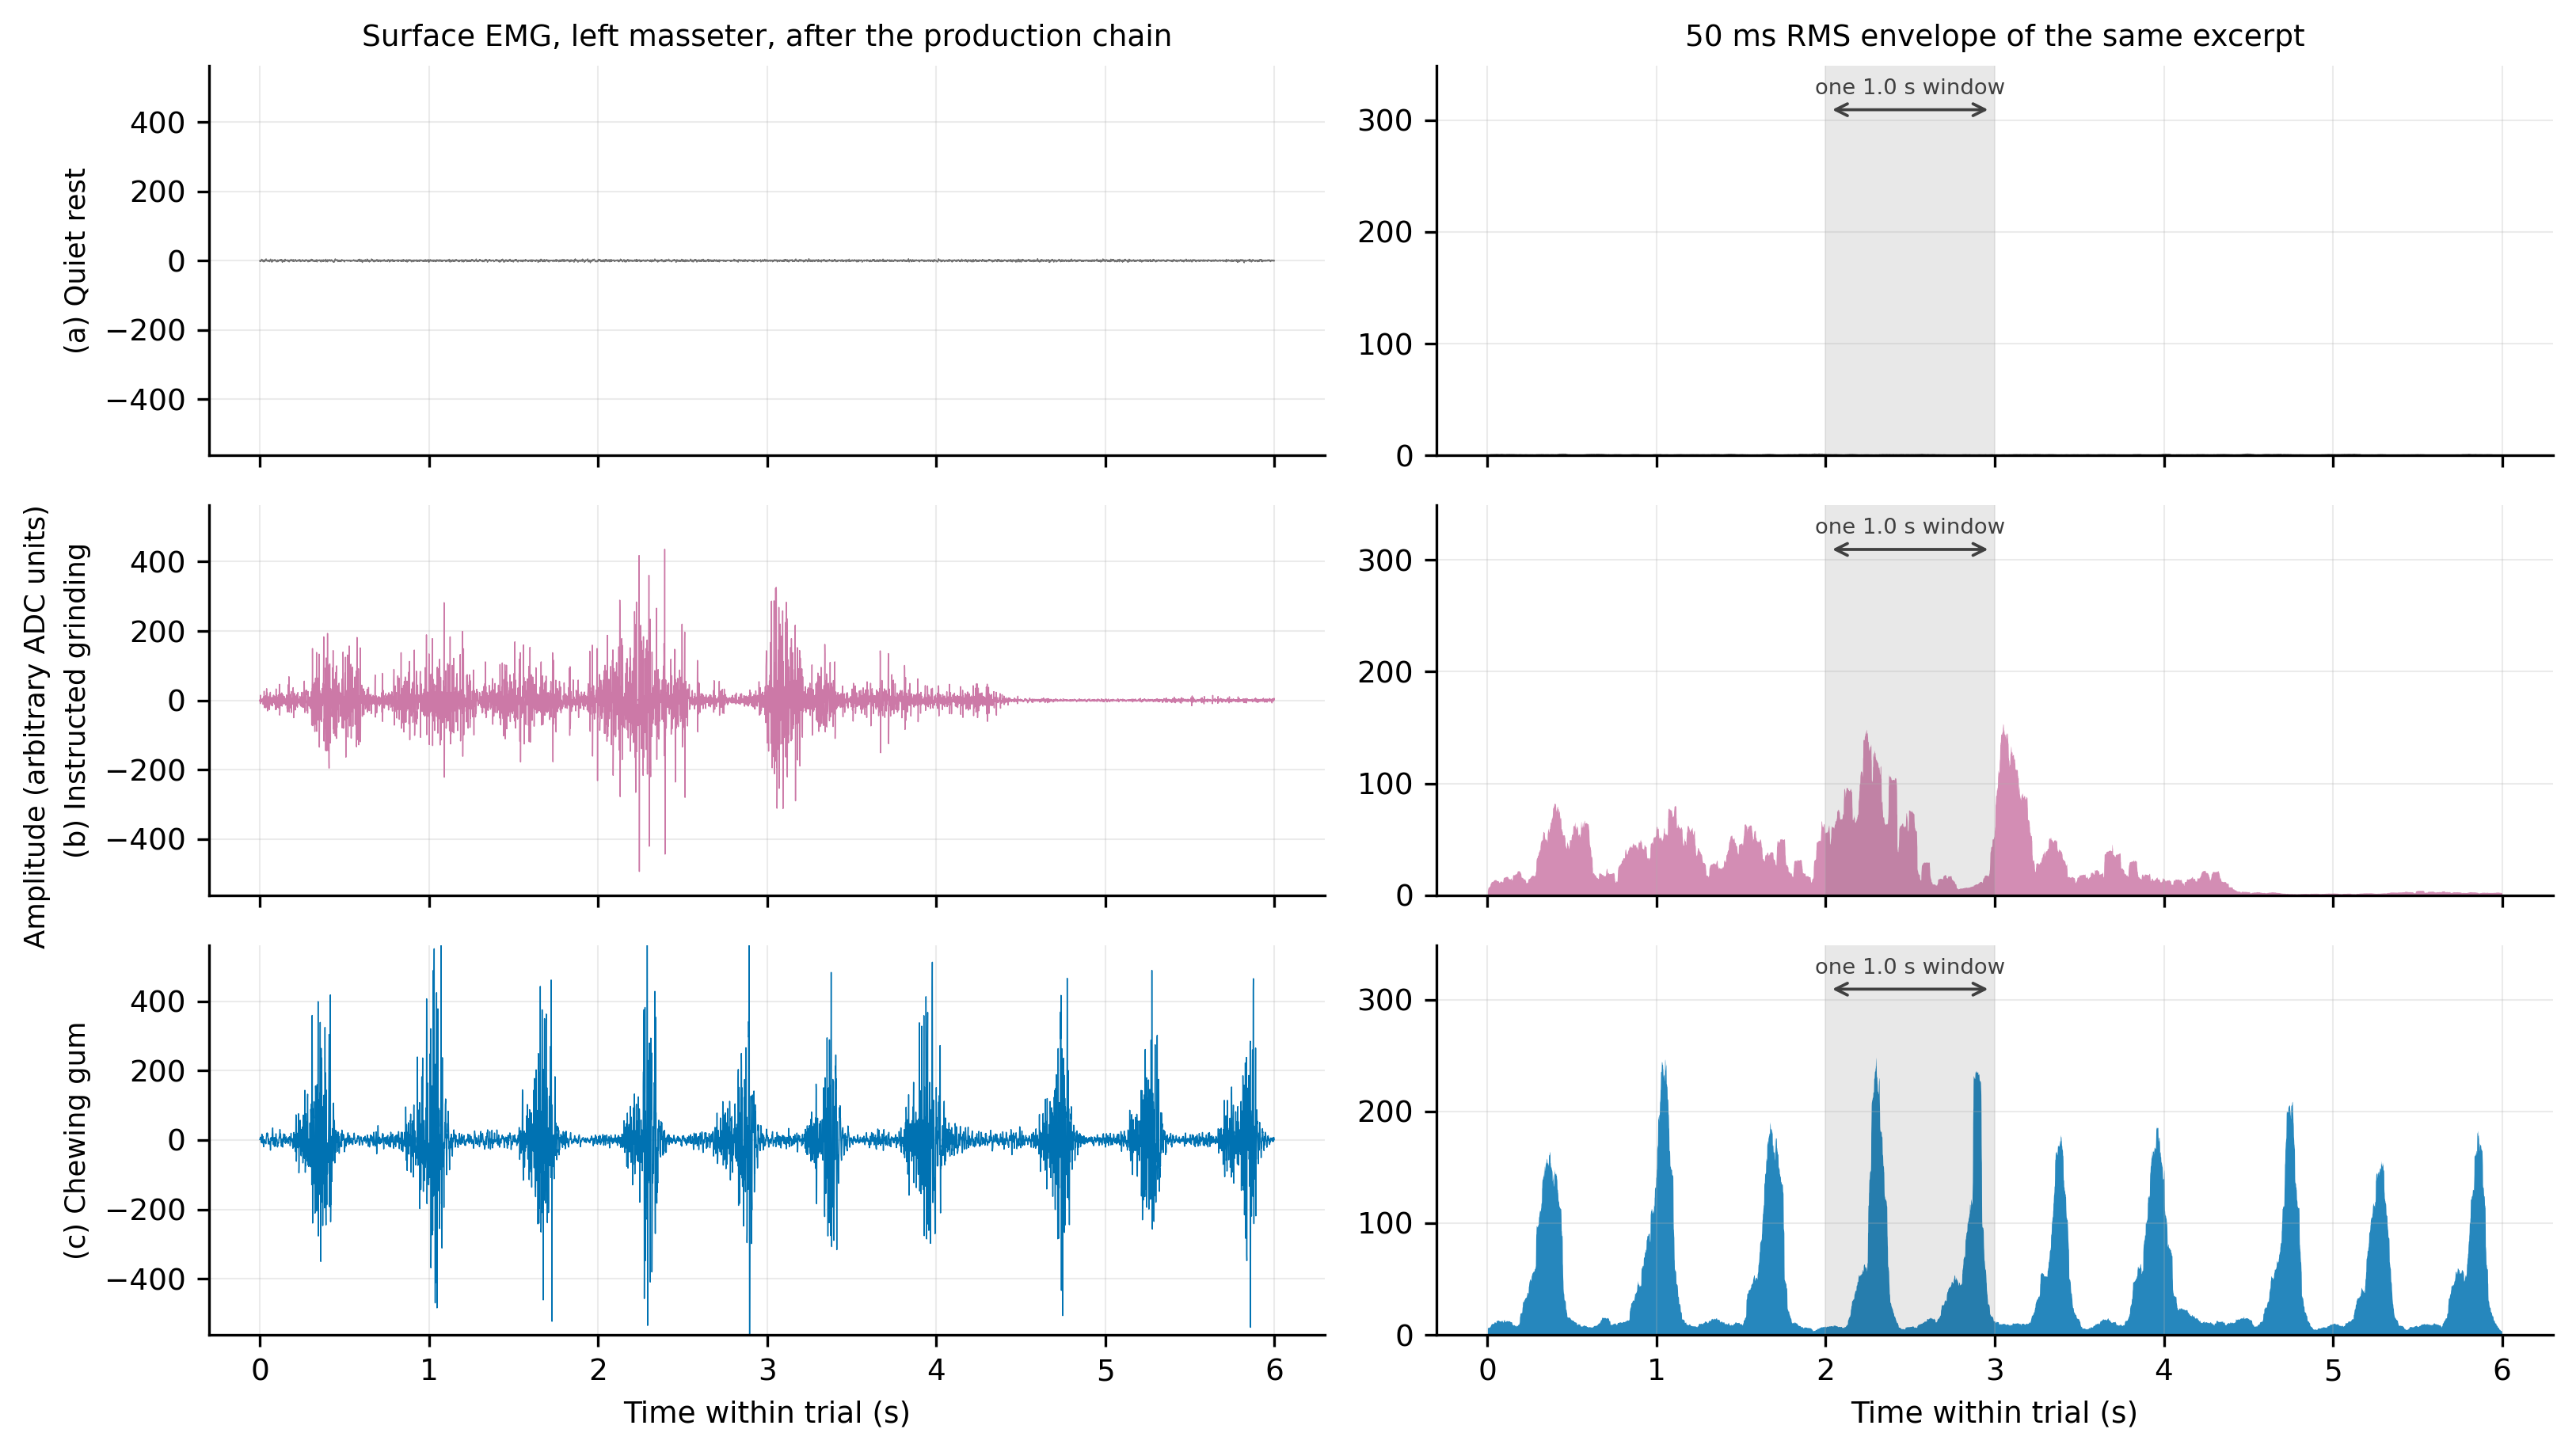
\includegraphics[width=0.68\textwidth]{Figures/v5/signal_comparison_emg.png}
  \caption{Six-second excerpts of one participant's quiet rest, instructed grinding and gum chewing after the corrected chain, on a common scale, with the 50~ms RMS envelope beside each. (a) Rest is quiet. (b) Grinding produces sustained activation without a clear burst and relaxation rhythm. (c) Chewing produces rhythmic bursts at roughly 1.4~Hz. The shaded interval is one 1.0-second analysis window to scale: it holds barely one chewing cycle.}
  \label{fig:signal_comparison}
\end{figure*}

\section{Training Behaviour and Computational Cost}
\label{sec:s_cost}

Because each fold's final model is refit for a fixed epoch budget chosen inside that fold, the curves in Fig.~\ref{fig:loss_curves} are training-fit diagnostics and the held-out participant appears in none of them. Training loss had largely flattened by the end of each budget, and the gap between training-fit and held-out macro-F1 averaged 0.144, largest for P1 at 0.276 and smallest for P5 at 0.040, an ordering that tracks the per-participant results of the main text: the signature of between-participant variation rather than optimisation failure. Three latencies must be kept separate: the input-context latency of 1000~ms, the window length; the decision interval of 500~ms, the stride; and the processing latency, a median forward pass of 1.02~ms for one window at batch size 1 on an Intel CPU for the compact model, 2.21~ms for the extended wavelet CNN, 0.20~ms for the early-fusion CNN and 1.16~ms for the bidirectional LSTM. None supports a real-time claim: no streaming implementation exists, the chain is acausal, and power and wearable reliability are unmeasured.

\begin{figure*}[!t]
  \centering
  
\includegraphics[width=0.64\textwidth]{Figures/v5/training_curves_5class.png}
  \caption{Refit training loss (a) and training-fit macro-F1 (b) for all fifteen fold and seed combinations, coloured by held-out participant; line style encodes seed. The held-out participant contributes to no curve and is scored once, after training ends.}
  \label{fig:loss_curves}
\end{figure*}

\section{Data, Code and Artifact Provenance}
\label{sec:s_provenance}

The datasets generated and analysed during the current study are not publicly available because of participant-privacy restrictions but are available from the corresponding authors on reasonable request, subject to institutional and ethical requirements. The archive holds, per recording, the six-column file as acquired, its metadata sidecar and the review video; the videos are identifiable and are not shared. The custom code for preprocessing, wavelet decomposition, training and evaluation is available from the corresponding authors on reasonable request. Every number and figure was regenerated from a saved artifact. The confirmatory five-class results come from the EMG conditions of run \texttt{modality\_and\_no\_chewing\_}\allowbreak\texttt{20260810T020642\_cead62e4} (configuration hash \texttt{cead62e4}, manifest \texttt{7ebbcc8d}, window index \texttt{b2cf690c}); the architecture sweep from run \texttt{baselines\_emg\_only\_20260816} (manifest \texttt{9d93667b}, window index \texttt{9941fe48}); comparing the two prediction ledgers window by window returns the identical 6,173 windows, labels and held-out assignments. The pre-correction contrast arm is the nested-LOSO run through the superseded chain on byte-identical windows. Parameter counts and latencies come from \texttt{outputs/benchmarks/}\allowbreak\texttt{benchmark\_emg\_only.json}. The confusion, ROC and per-participant panels depict one trained model per fold at the lowest seed index, a fixed rule rather than a choice made after seeing the scores.

\section{Author Contributions}
\label{sec:s_contrib}

M.H.F.: methodology, software, analysis, writing---original draft, and writing---review and editing. A.R.: protocol development, software, data curation, data collection, formal analysis, and review and editing. R.S.: methodology, validation, and writing---review and editing. M.P.F.: conceptualization and study design, research-grant development, protocol development, and manuscript revision. R.A.: conceptualization, project administration, resources, supervision, and writing---review and editing. T.A.W.: conceptualization, research-grant authorship, protocol development, project oversight, and manuscript revision. All authors reviewed and approved the final manuscript. The authors declare no competing interests.

\bibliographystyle{IEEEtran}
\bibliography{refs_v8}

\end{document}
